\documentclass[11pt,conference,a4paper,onecolumn,romanappendices]{IEEEtran}
\usepackage[utf8]{inputenc}
\usepackage[english]{babel}
\usepackage{verbatim}
\usepackage{graphicx}
\usepackage{wrapfig}
\author{Lucas Colantuono, Lucas Kummer, Shanan Lynch, Samuel Sedlmeir}

\title{IoT Trace Analysis}
\date{\today}
\markboth{Improving local transports by analysing taxi meta data}{}

\author{\IEEEauthorblockN{Lucas Colantuono}
\IEEEauthorblockA{INSA Lyon \\
lucas.colantuono@insa-lyon.fr}
\and
\IEEEauthorblockN{Lucas Kummer}
\IEEEauthorblockA{INSA Lyon\\
lucas.kummer@insa-lyon.fr}
\and
\IEEEauthorblockN{Shanan Lynch}
\IEEEauthorblockA{INSA Lyon\\
shanan.lynch@insa-lyon.fr}
\and
\IEEEauthorblockN{Samuel Sedlmeir}
\IEEEauthorblockA{INSA Lyon\\
S.Sedlmeir@campus.lmu.de}}

\begin{document}

\maketitle

\tableofcontents
\newpage

\begin{abstract}
 
\end{abstract}

\section{Introduction}
\label{sec:Introduction}
\begin{comment} All over the world big cities are struggling to fight against air pollution as a result of individual transport. This does not just concern developing countries or emerging countries, but also developed first world countries: Beijing will ban certain cars to prevent an overriding of the emission limits \cite{beij}, whereas the city of Oxford is planning to establish a petrol car free zone \cite{oxfo}. \\
While bans forbid people to use their cars, a more sustainable way would be to make people use the local transport voluntarily by improving it where necessary. Thus we need a reliable possibility to learn about people's possible needs. As a lot of people choose a taxi where there is a unsatisfying offer of transport, we could use taxi meta data in order to analyse automatically possible useful routes for new bus lines for example. \\
To achieve this goal, we use data collected by taxis in Shanghai in 2007. These data contain GPS positions, a timestamp, the status, the direction in which the taxi is moving as well as a Taxi ID. In order to analyse this data we set up a InfluxDB Database and a Chronograf and Grafana Web Server, where the data is being inserted to by using a Python script.
\end{comment}
\section{Related work}
There are several different articles, that analyse the same dataset.
\section{Data consistency}
The first task is to check and improve the consistency of the provided data. Therefore we will use R and Python. \\
At the beginning we have to filter all impossible values of the variables we're operating on. For example, our R script removes all entries with a negative speed value or timestamps outside of the interval in which these data have been collected.  Apparently the trace files only contain consistent data sets as our script has not detected and removed a single error. \\
Furthermore, there are two more types of errors that have to be considered: Checking the geographical consistency and filtering gaps in the traces.
\subsection{Geographical consistency}
The next step is to filter the data by the coordinates. As we decided to focus on the city centre, we only keep those entries in our dataset that have a longitude between 121.38 and 121.57 and a latitude between 31.15 und 31.32. In figure \ref{fig:borders} you can see our chosen borders on a map with around 19.000 randomly chosen points.\\
\begin{figure}[h]
\centering
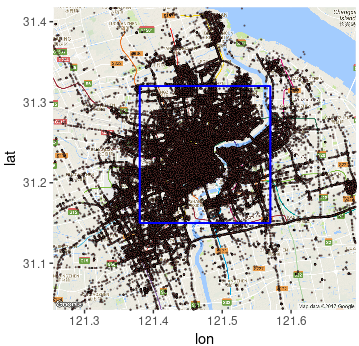
\includegraphics[scale=0.9]{borders.png}
\caption{\label{fig:borders}Borders of the city center}
\end{figure}
Second, we analysed several statistical metrics concerning the speed variable which showed that there is a wide spectrum of different values, with some outliers bigger than 200 km/h, which does not make any sense in a city centre and is probably an error. Thats why we decided to cut off all the entries with a speed higher than three times the interquartile range. As you can see in figure \ref{fig:speed} the speed distribution is skewed right with a single maximum. That justifies our decision, because we don't lose relevant data entries, when we choose our cutoff speed value. \\
We also observed that limiting the data to the city center changes the speed distribution, as some streets outside don't have a low speed limit. For example we lost some data entries on the street towards one of the airports by removing all the points with a speed higher than 80 km/h. \\
\begin{wrapfigure}{r}{0.5\textwidth}
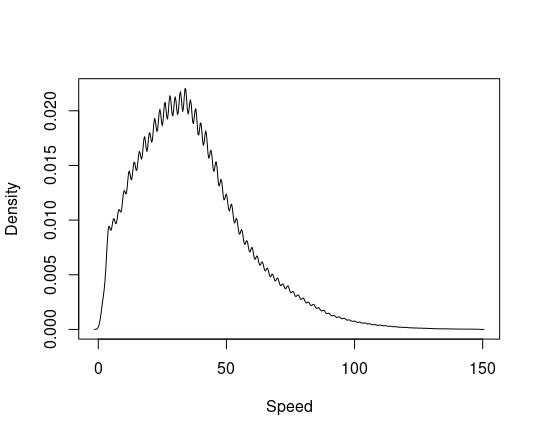
\includegraphics[scale=0.67]{speed.png}
\caption{\label{fig:speed}Adapted speed distribution without zero values}
\end{wrapfigure}
\subsection{Gap filtering}
After this procedure we are already able to plot a schematic map of Shanghai, although a dataset still contains a lot of data to be removed. We make use of Python to find those taxi traces with a time gap between two data entries. This gap could either be a result of a data transmission error or an indicator for the beginning of a new taxi trip.
\section{Analysis}
\section{Results}
\section{Summary}

\newpage
\bibliography{biblio}
\bibliographystyle{IEEEtran}

\end{document}